%----------------------------------------------------------------------------
\appendix
%----------------------------------------------------------------------------
	\chapter*{F�ggel�k}\addcontentsline{toc}{chapter}{F�ggel�k}
	\setcounter{chapter}{6}  % a fofejezet-szamlalo az angol ABC 6. betuje (F) lesz
	\setcounter{equation}{0} % a fofejezet-szamlalo az angol ABC 6. betuje (F) lesz
	%\numberwithin{equation}{section}
	%\numberwithin{figure}{section}
	%\numberwithin{lstlisting}{section}
	%\numberwithin{tabular}{section}

%----------------------------------------------------------------------------
%\section{Fut�si eredm�nyek}
%----------------------------------------------------------------------------

	\begin{figure}[!ht]
		\centering
		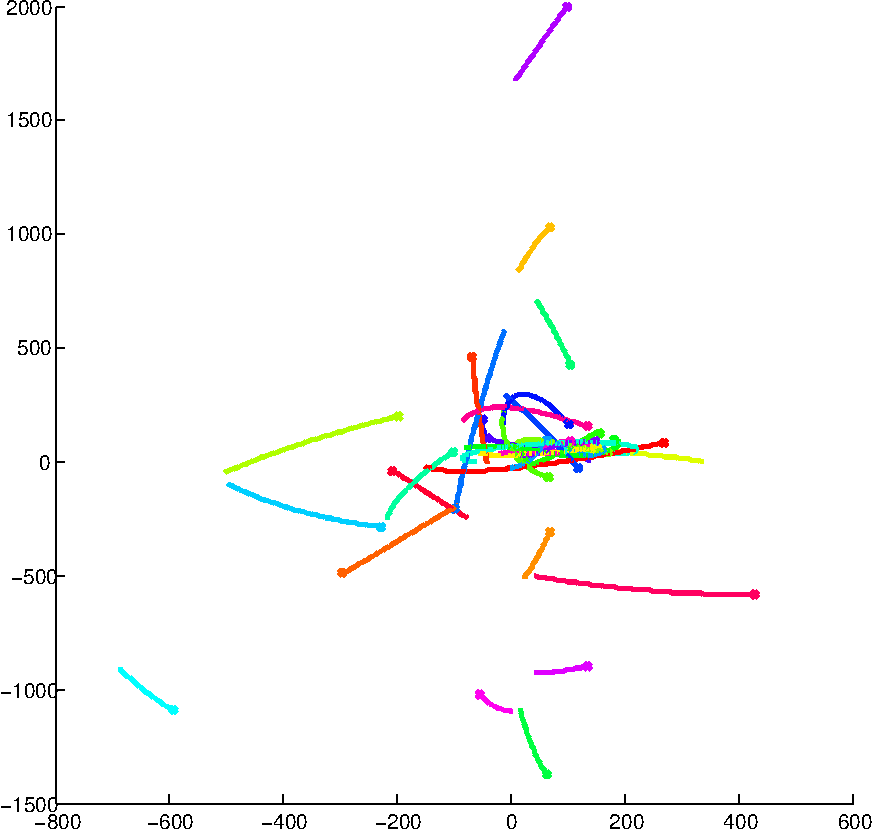
\includegraphics[width=150mm, keepaspectratio]{figures/MATLAB/32_direct-cropped.pdf}
		\caption{Direkt algoritmus �s saj�t integr�tor fut�si eredm�nye MATLAB-ban}
		\label{fig:32_direct}
	\end{figure}
	
	\begin{figure}[!ht]
		\centering
		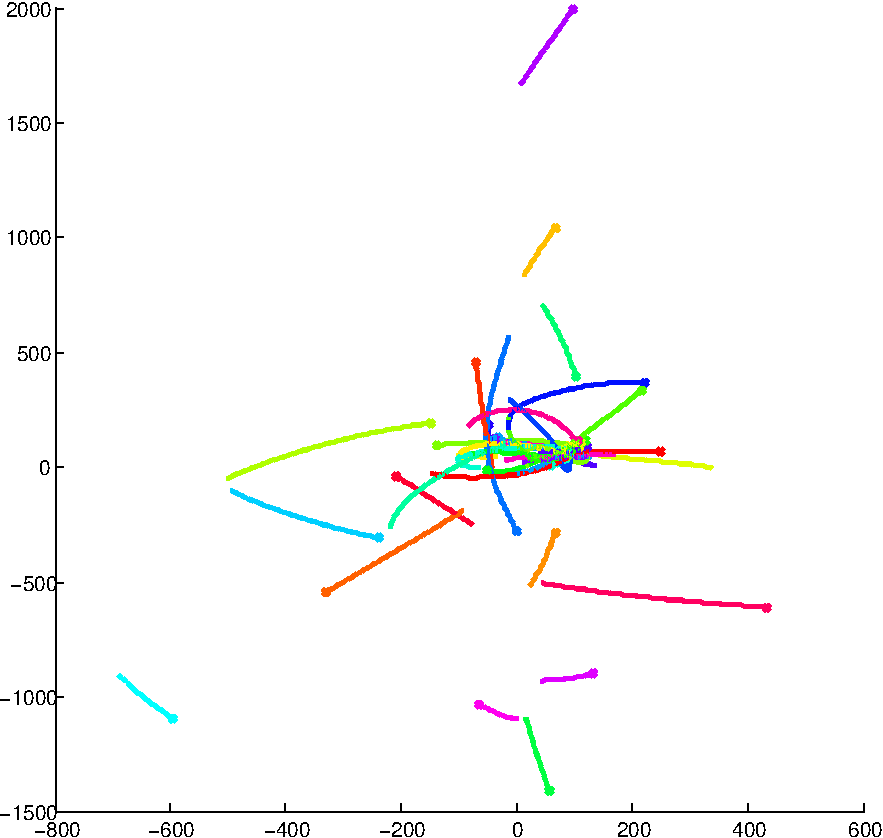
\includegraphics[width=150mm, keepaspectratio]{figures/MATLAB/32_ODE-cropped.pdf}
		\caption{Direkt algoritmus �s KDE megold� fut�si eredm�nye MATLAB-ban}
		\label{fig:32_ODE}
	\end{figure}
	
	\begin{figure}[!ht]
		\centering
		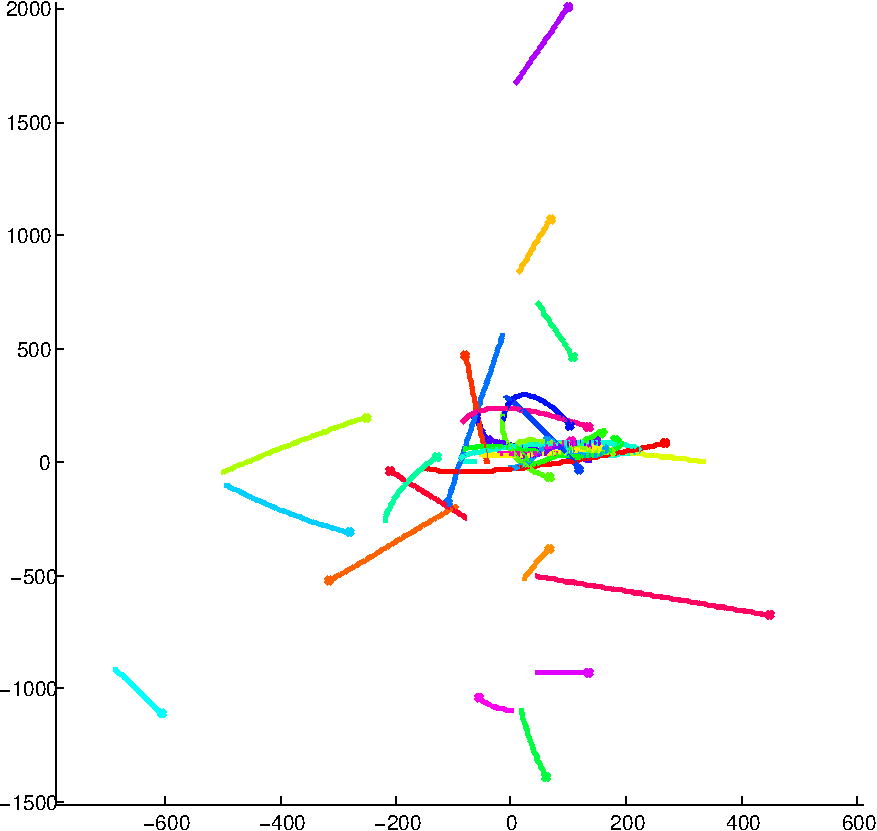
\includegraphics[width=150mm, keepaspectratio]{figures/MATLAB/32_selective-cropped.pdf}
		\caption{K�zel�t� direkt algoritmus �s saj�t integr�tor fut�si eredm�nye \mbox{MATLAB-ban}}
		\label{fig:32_selective}
	\end{figure}


	\begin{figure}[!ht]
		\centering
		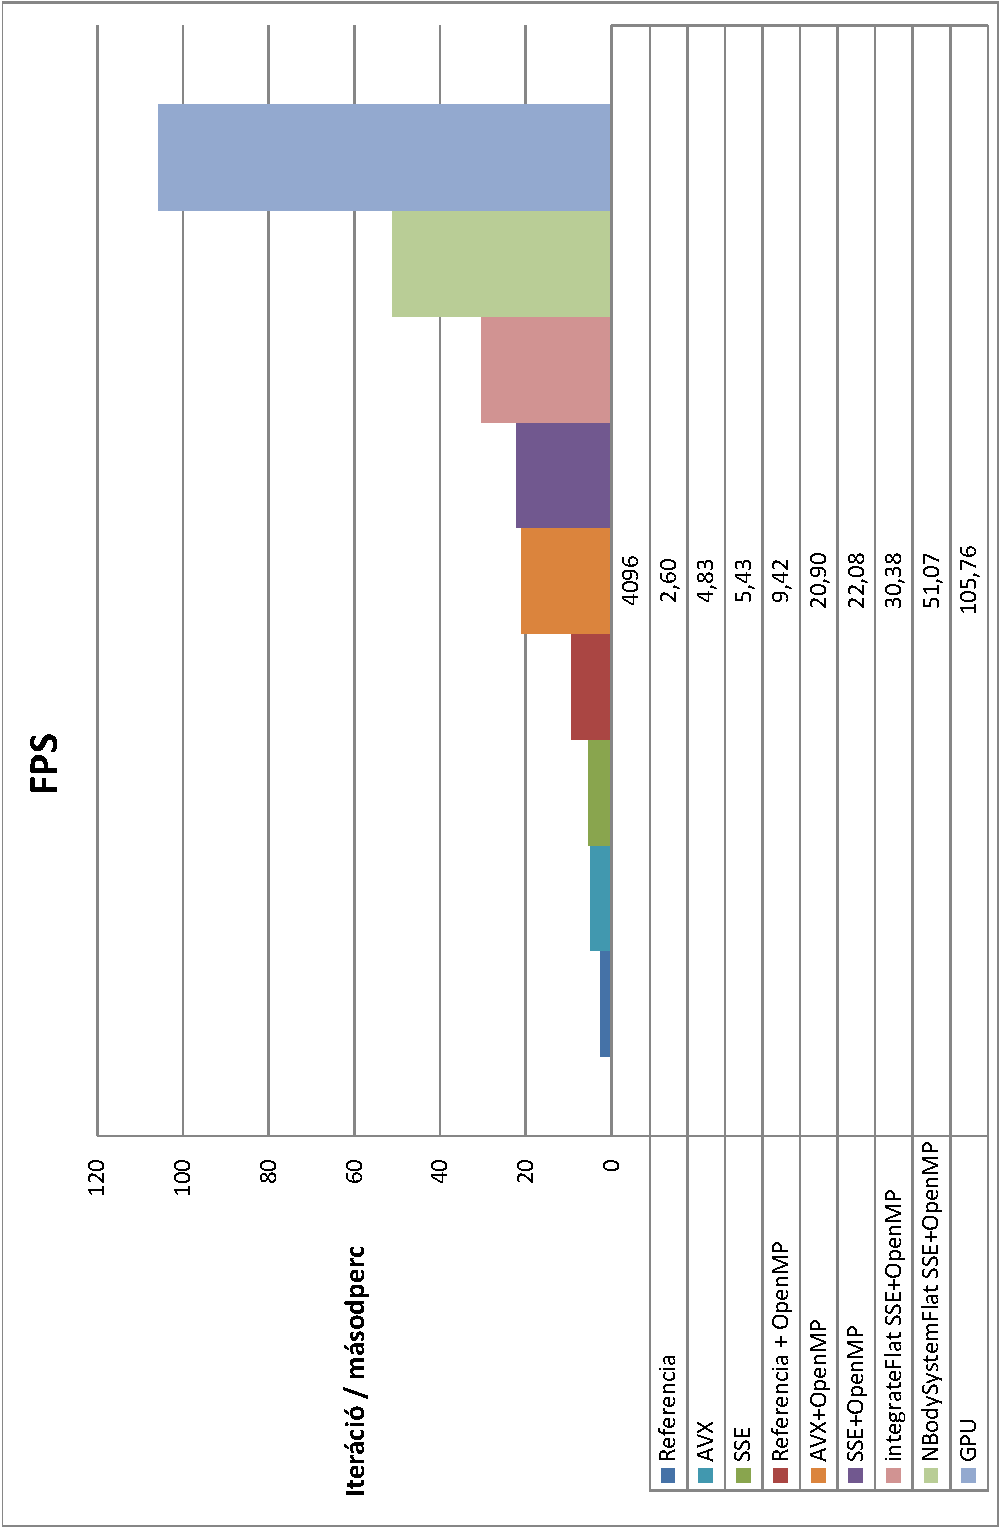
\includegraphics[width=150mm, keepaspectratio]{figures/Performance/FPS-cropped.pdf}
		\caption{Frame rate 4096 test eset�n}
		\label{fig:Perf_FPS}
	\end{figure}

	\begin{figure}[!ht]
		\centering
		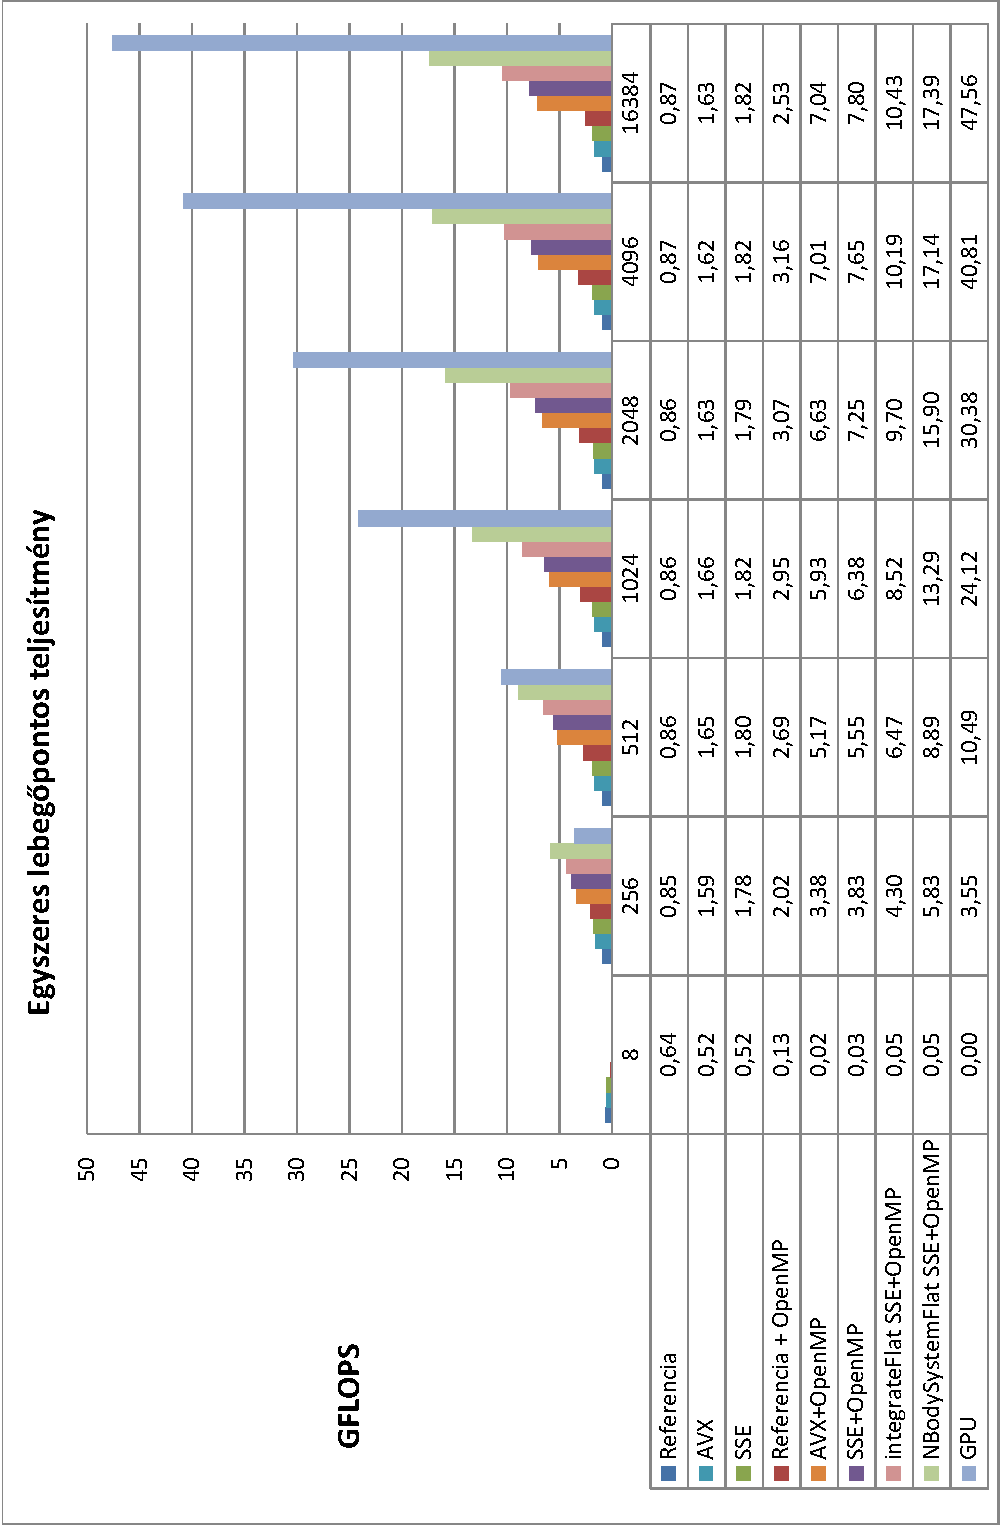
\includegraphics[width=150mm, keepaspectratio]{figures/Performance/GFLOPS-cropped.pdf}
		\caption{K�l�nb�z� konfigur�ci�k sz�m�t�si teljes�tm�nye}
		\label{fig:Perf_GFLOPS}
	\end{figure}

	\begin{figure}[!ht]
		\centering
		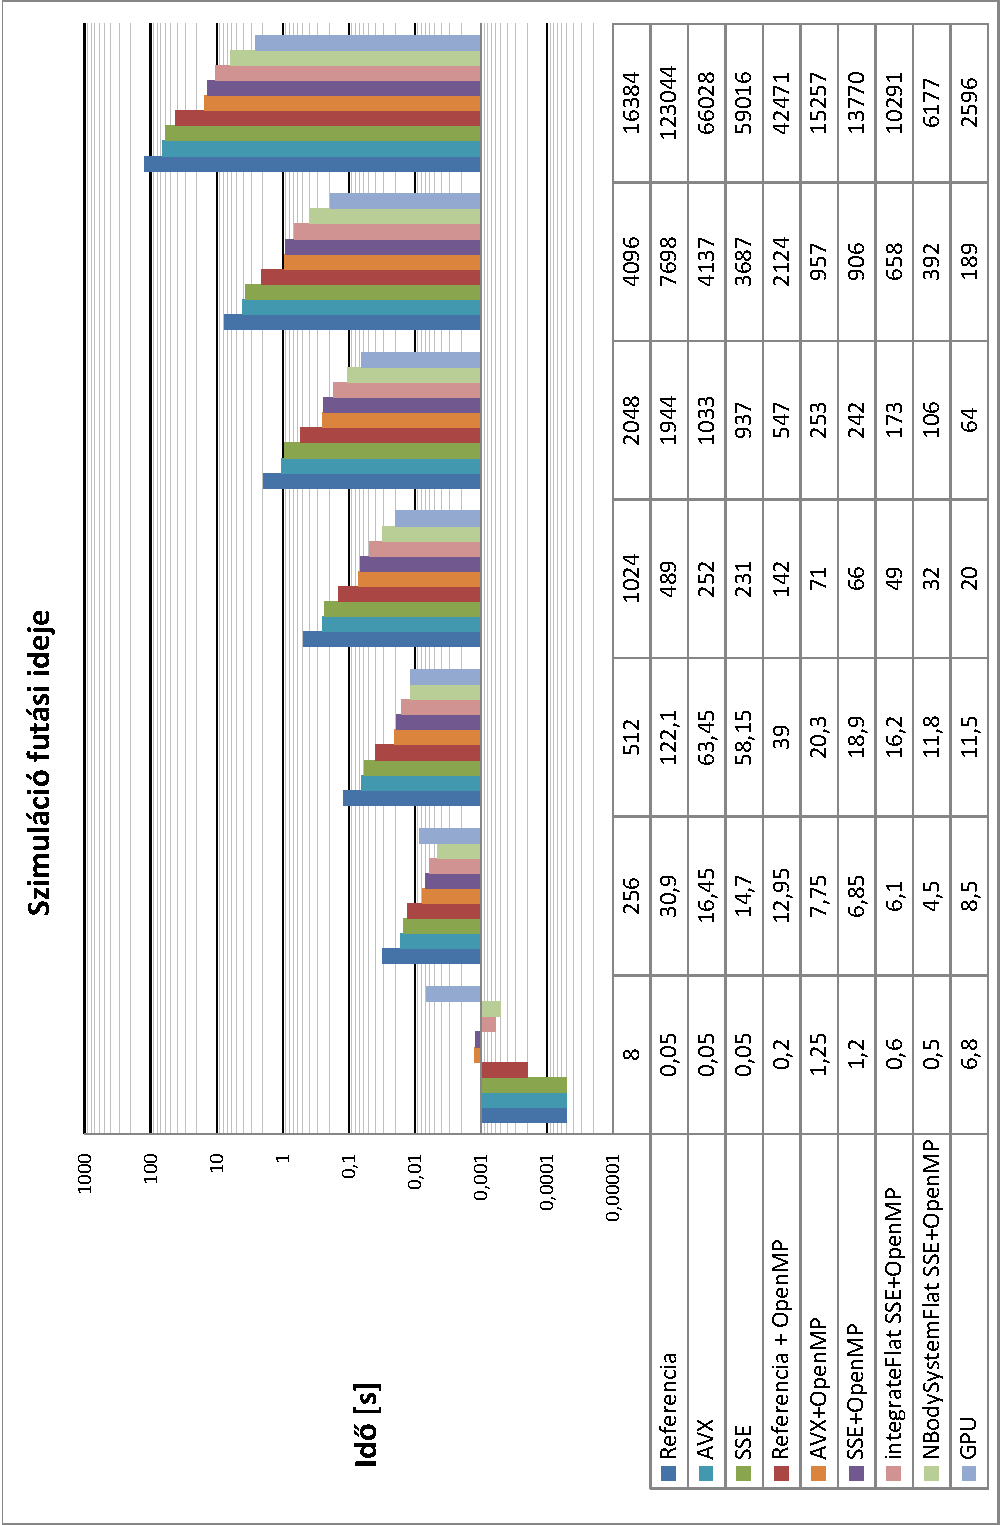
\includegraphics[width=150mm, keepaspectratio]{figures/Performance/FUTAS-cropped.pdf}
		\caption{K�l�nb�z� konfigur�ci�k fut�si ideje}
		\label{fig:Perf_FUTAS}
	\end{figure}
	
	
	
	